\appendix
\chapter{Journal}
\section{Day 1}
\begin{tabular}{|c|c|}
\hline
Date: & 07.10.2013 \\
\hline
\end{tabular}
\subsection{Traveling}
\subsubsection{Bus}
I started out with waking up at 05:00am. Usually I get my salary from Peppes at the 7th each month, but this time there was a delay.
So waking up, I was broke. No money for the Planebus. I tried to get some money from the local gas station with my mastercard with no luck.
With only 3minutes until my bus was leaving i hoped that the bus driver would accept my mastercard. He did.
Either way i was in luck, just before I was going to pay i checked my balance and my salary was in.
\subsubsection{Trondheim Airport}
No problem here. Talked a little with my mom, said goodbye and registrered. Plane ride was good.
\subsubsection{Oslo Airport}
Met up with Simen. There was some problems with he's visa. One cannot leave Norway and have a visa that expires before your return date.
He had fortunately bought a flex ticket so he could just change the dates, and then change them back when he arrives Kigali and prolonges his visa.
Then it was off to Istanbul. Flight was ok, good movies.
\subsubsection{Istanbul}
A little short on time. Didn't find the directions to our gate at first. The signs were properly hidden. After a little exploring we found it. Next stop, Kigali.
The flight seemed a little longer, but it was cured by `free cell' and `soduko'.
\subsubsection{Kigali}
At last, after about 18 hours from Trondheim, I was here. The guy that checked out our visa seemed a little sceptical, asked me one more time of my purpose of visit.
I just explained that we had an internship with the Management Sciences for Health and it was ok.
Felix picked us up and drove us to our house, 21KK Avenue, Niboye Road.
Awsome house! Randy's old place. We could stay here for free out October.
Took a beer with Felix and went to bed.
\section{Day 2}
\begin{tabular}{|c|c|}
\hline
Date: & 08.10.2013 \\
\hline
\end{tabular}
\subsection{Meeting with Randy}
\subsubsection{Breakfast}
Got off to a bad start today. Woke up 10:05AM and we were expecting Randy at 10:00AM. No worries though, he wasn't there yet.
Took a shower. Simen sat outside talking to our day-time guard, Peter.
I took some breakfast, bread with jelly, a tomato and a banana. The bananas here are very small. Anyways, Randy came in the middle of breakfast and we talked some.
\subsubsection{Bank}
Then we drove out to the bank. About a 5 minute drive I think. We took out 100 000RFR, this should cover us for about 2 weeks Randy said. About 1000NOK.
Then we had to get our SIM-cards.
\subsubsection{MTN}
Pretty straight forward. We registreded our passports and got our sim cards with unlimitided data usage.
\subsubsection{Lunch}
We got liuch at a chiniese resturant. The food was not very great, but better than airplane food I think. Strong chilli. We got chicken, goat and some vegetables.
Simen and Randy were so kind and decided that for me.... 
We then got to talk about the project. In general I think we got 3 options.
Malarya registration by phone, system migration from Voxivia and a bigger project that involved several Systems and a Data warehouse.
The systems included HMS, Inidcator Remarks and health finances. The data warehouse should also be able to pull data from several instances.
We did not land on a specific one and we were presented with some other options as well.
The project that involved several instances had alot of subproject bound to it.
Andrew is the system wizard, Eric the doctor that likes his ways and Beth is a eager IT-person.
Randy talked a little about another survey that he thought was better than DHIS2. We should gather some recomendations here I think.
\subsubsection{The Office}
Then we went down to the office were we will probably work. Our space consists of 4 cubicals that we share with 2 others.
It was not far from the ministry of health.
\subsubsection{Back Home}
Randy had to go to a meeting so we called it a day. We were invited to join a training program on thursday later this week. Meeting up with Randy 08:30AM tomorrow.
\section{Day 3}
\begin{tabular}{|c|c|}
\hline
Date: & 09.10.2013 \\
\hline
\end{tabular}
\subsection{First day at the office}
We were drown from our house to the ministry of health by Randy today. 08:30AM. Early day. Randy had some meetings and we've got the oppertunity to chack our emails and catch up on some reading. I found some new articles today that talked a little about how there is a gap between some countries in the IT world. Talked a little with Simen about ttrying to share our perspectives to get the best from both worlds.
\subsection{DHIS2 Intro}
After a while Randy was finished with his meetings. Andrew, the system wizard, came and said hello. He is joining us tomorrow for some DHIS2 training.
We where introduced to alot this session. Mostly about how they were using DHIS2 today. DHIS2 is not the only program they use. The functionality that are needed, but not supported by DHIS2, are hacked into their day-to-day work with some scripts made up by different people. I think their data is pushed to the server monthly. \\
Here is some changes that Randy suggested.
\begin{itemize}
\item Wanted to make some good validation rules, but lacked people with experience in the field to make them proparly.
\item After the usercount got high, the favorites got very messy and unorganized.
\item Would like to share tables, diagrammes and maps with individuals and make only a selected few public.
\item Some labels on the map, didnt quite get that one.
\item They would like to choose what type of faccilities that would be viewed in GIS. This would be a great improvement.
\item They had some language barriers. Would like som improbements there. Didnt get the details.
\item Problem with reports being loaded from NGINX cache, they were not updated after changes if it already was in NGINX cache.
\end{itemize} 
I was wondering how he trusted the data. It turned out that sometimes the data wasnt accurate. This was tested by some people motivated by a Performance Based Finance system. The health facilities down here get some funding based on their registration count. Some cases are worth more than others. Like, dont actually know the numbers, but lets say 1000RWF for registrating a pregnant woman. So to prevent health facilities from cheating the authoreties take some samples in order to check if the inputed data is correct. Randy would like some more competance on iReport. Should check that out later. FOSAID is the identification number used through all the databases. This identifies the facility. This number is also used by external systems. I think I should get a better understanding of Pivot tables. They are quite popular here. Camel is used to make an access level from the MOH to extarnal systems.\\
He also gave us an overview of how everything should be linked together in the future.\\
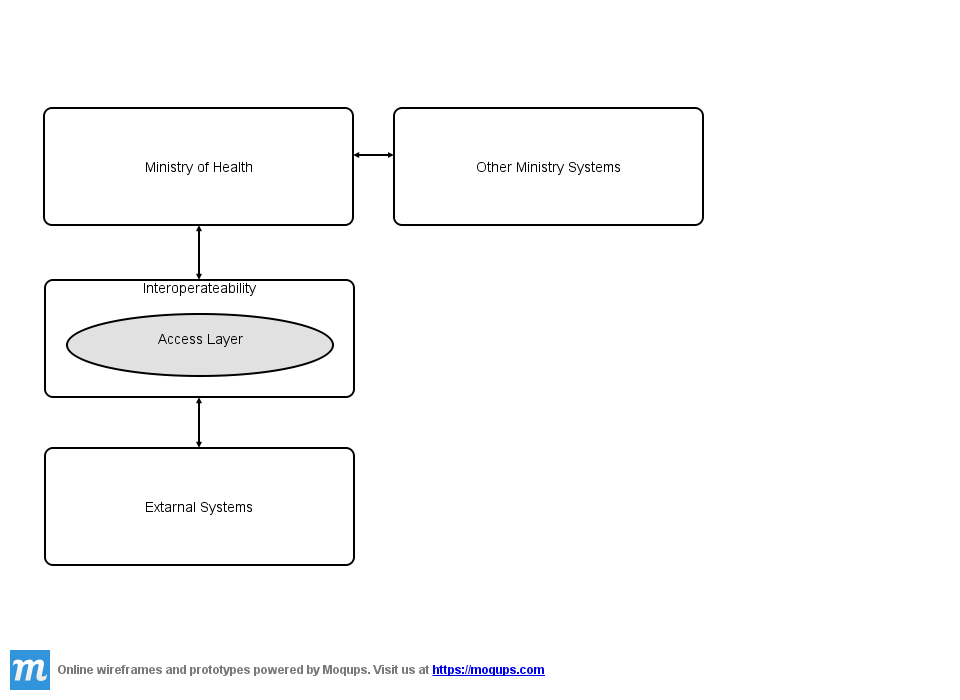
\includegraphics[width=15cm]{appendix/images/future_design_rwanda}\\
I then wondered how they could trust the open source code to do its job. Is there some testing that ensures that DHIS2 is working as it should? To me this seems like life or death for some people. When funding is based on registration of data. Is this the only option that MSH have? What other options did they consider before DHIS2? And what was the primary factor for choosing DHIS2. Open source? Proprietary softerware alternatives? I know I would be very sceptical to a software that did not guarantee customer support. 
\subsection{Lunch}
During luch we got some food from a burger diner. Good food, bad smell around the toilet. Randy just had a baby that is 4 months old with his second wife from Rwanda. She had family in Trondheim and visited them not to long ago. 
\subsection{Install Rwanda DHIS2}
When we got back we installed all the necesarry software. We got our own copy of the database so that we could work localy on our machines.
\begin{enumerate}
\item JDK
\item Postgres
\item Ireport
\item Tomcat
\item odbc
\item restore database
\item edit hibernate.properties
\end{enumerate}
I think I should get more comfortable with enviroment variables in Windows. 
I should get back to my todo list for sure.
\subsection{Dinner}
After work we ate at a Italian resturant. A little bit pricy. Should probably find some cheaper alternatives.
We are getting picked up at 07:30AM tomorrow, so I should probably get some sleep now. Good NIGHT!
\section{Day 4}
\begin{tabular}{|c|c|}
Date: & 10.10.1987 \\
\end{tabular}
\subsection{1st session: Review of training}
The datamanagers from different facilities reviewed their previos training. See email from Gloria for more information.
Wheres the map? (Because they removed it.)\\
Inser chart list maybe to long.\\
Why is the top border gone in gis? (Problem solved)\\
Wheres the back button? (Found it!)\\
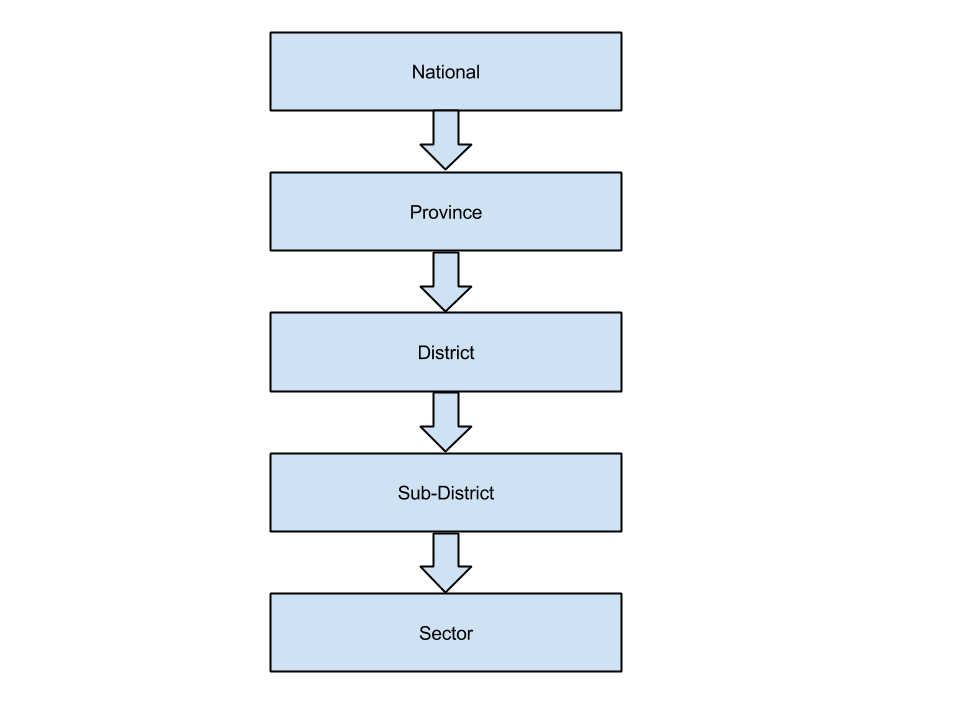
\includegraphics[width=15cm]{appendix/images/dhis2_map_categories}
\subsection{Meeting}
We talked a little bit here in order to get a better understanding of how they used the DHIS2. The consisted of me, Simen, Gloria, Adolf and three other data managers. It was a little difficult at first, but after a while I think we've got a pretty good understanding of it. They use DHIS2 for data analyses and for reporting data. Reporting data is done by the data manager at each health facility. Data analysing is used by monitoring and evaluation officer and head of community officers for decision making and strategic planning. \\
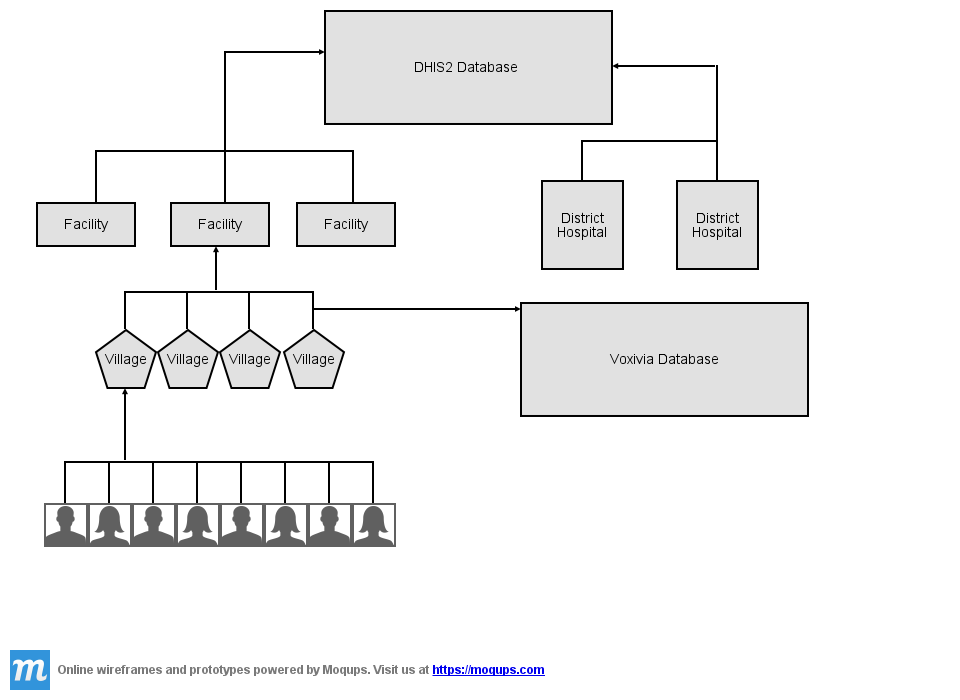
\includegraphics[width=15cm]{appendix/images/Dataflow} \\
The collecting of data starts in paper form. They are then gathered at each facility for reporting in the DHIS2 database. They have a seperate reporting system with voxivia. They still use this because they allow for more detailed information. If they use DHIS2 they have to track the reporting to the paperbased forms in order to get the ground details. Adolf mentioned that he would like a way to combine the data from the tracker and the aggregated data. This was a nice feature that they would like.
\subsection{Dinner}
Dinner was awsome!
\subsection{Second Session}
We then had a look at their presentations. We only stayed for one presentation. Then it was photo's. Thumbs up Simen!
\section{Day 5}
\begin{tabular}{|c|c|}
\hline
Date: & 11.10.2013 \\
\hline
\end{tabular}
\subsection{MSC Office}
We set up at the Management Sciences of Health office. We met alot of new people. Mircel, I don't really know what he does yet. Think it was finance. Felix, good to meet him again. Bob the american. Cedrick and Emmir. Cedrick is a little shorter than Emir. And some other people.\\
\begin{figure}[p]
\centering
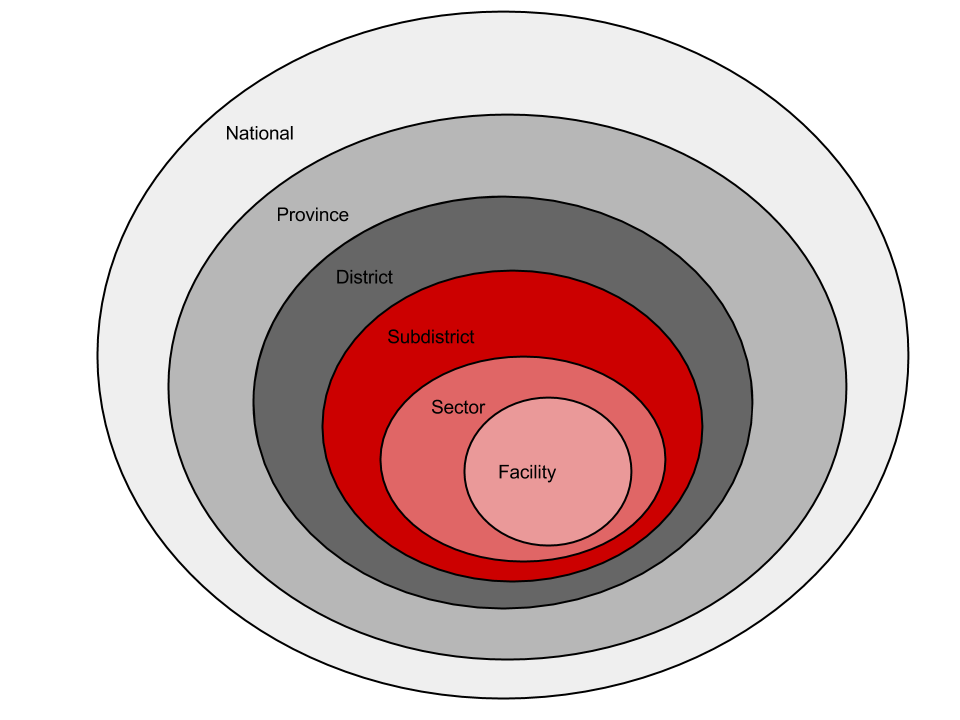
\includegraphics[width=15cm]{appendix/images/dhis2_rwanda_map_hierarchy}\\
\caption{Rwanda Map Hierarchy in DHIS2}
\label{Rwanda Map Hierarchy in DHIS2}
\end{figure}
\subsection{After Brunch}
After Randy's meeting we talked a little more about the projects that are relevant. The malaria surveliance and the interoperateabillity. I want the Malaria Surveliance. This would give us a concret assignment and a `know when its done' thing. The interoperateability would probably give us the best learning experience. Because it challenges me to think at computer systems at a higher level. I will send an email to Eric and discuss it further. I have a feeling I wont enjoy the best choice. Nappolina is the project manager.
\subsection{Conference room}
Randy gave us a briefing about the 2 remaining projects. This was alot of information to take in. 
\subsubsection{Malaria Active Surveliance}
The want to copy an existing report to a web based solution. Where this should be, I do not know.
\begin{itemize}
\item HTML
\item DHIS2
\item Mobile SMS
\item App
\end{itemize}
This was an extensive report. Randy proposed that we should mayby trim down the report a little. I think we've got the report on an email.
\subsubsection{Sentinal Surveliance}
This system is awsome. It's purpose is to collect weather and malaria data in order to see if theres an corelation between the two. They are going from 11 to 16 sentinels nationally. 
\begin{figure}[p]
\centering
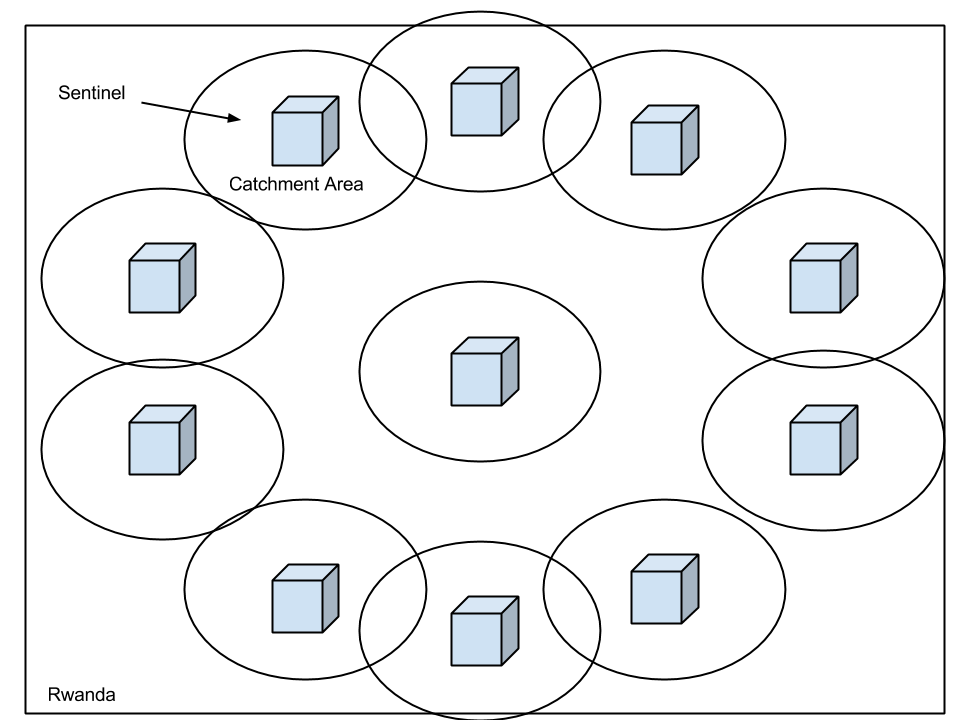
\includegraphics[width=15cm]{appendix/images/sentinel_surveliance}
\caption{Sentinel Surveliance}
\label{Sentinel Surveliance}
\end{figure}
\subsubsection{Ineroperateability}
Then got of to discuss the interoperateability project.
For starters Randy wanted to make a report based on some choosen indicators.
The task goes something like this.
\begin{enumerate}
\item Load data from dictionary
\item Choose indicators
\item Choose metadata/attributes
\item Produce report (Maybe with a preferred layout)
\end{enumerate}
He then explained how he wanted the entire system to work.
The result would be something like this.
\begin{figure}{p}
\centering
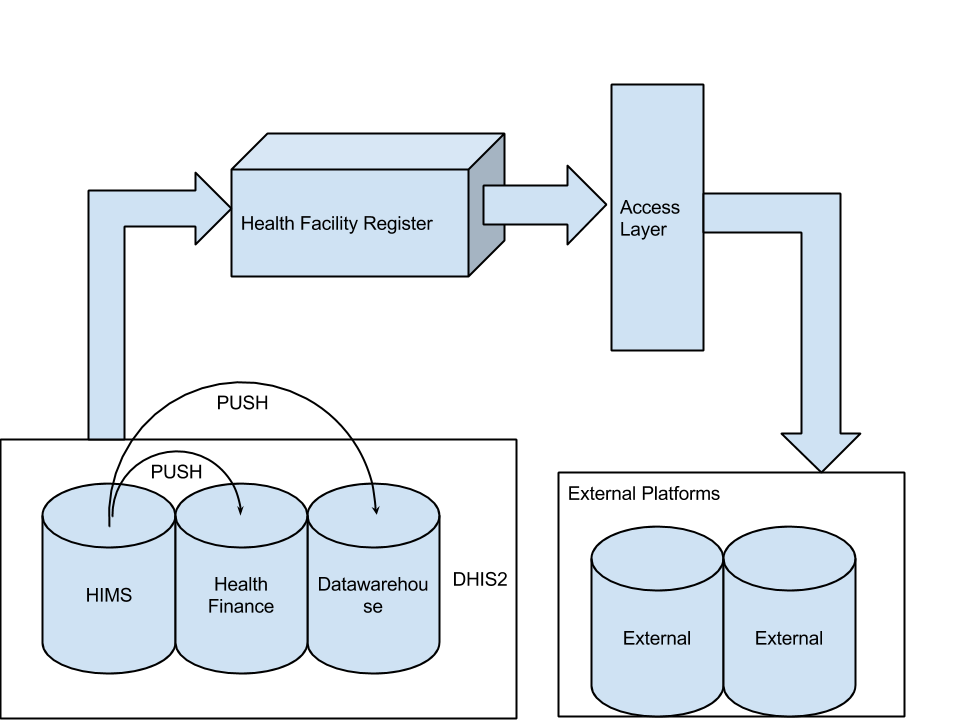
\includegraphics[width=15cm]{appendix/images/System_Architecture}
\caption{System Architecture}
\label{System Architecture}
\end{figure}
I think I should reaad up on SQL. It seem that this would be relevant.
For the last part he talked about how he would like to synchronize changes made to certain data element groups, cross instances of DHIS2. This in the case of adding adding elements. Would he like the same thin for indicators, I do not know. 
\subsection{Dinner at Randy's}
\section{Day 6}
\begin{tabular}{|c|c|}
\hline
Date: & 12.10.2013 \\
\hline
\end{tabular}
\subsection{HASH}
\subsection{Papairus}
\section{Day 7}
\begin{tabular}{|c|c|}
\hline
Date: & 13.10.2013 \\
\hline
\end{tabular}
\subsection{Spaghetti Dinner}
\section{Day 8}
\begin{tabular}{|c|c|}
\hline
Date: & 14.10.2013 \\
\hline
\end{tabular}
\subsection{Zero Values}
Today we got working on fixing  a database that had accedently deleted some 0's. Randy want to delete all zeroes from a specific date and then insert the ones from the last week or so. I thought this should be done directly with the database. This worked fine, but resulted in dates being placed instead of a NULL. I think this is very wrong. Should probably mention that we had a problem with the dataset. The booleans and the dates where not always present. This caused POSTGRESQL to stop when we tried to import the data. So Randy filled in all the empty values. This resulted in the same way as the other way.
\section{Day 9}
\begin{tabular}{|c|c|}
\hline
Date: & 15.10.2013 \\
\hline
\end{tabular}
\subsection{Before lunch}
We've just had a solution. We first import the data that should be updated. Then we import data with the right zeros. We then select the records that should be updated and do so. NP I think..... I think the only troubling part is learning how to use SQL and the operating system. On thing should be mentioned before I forget. There is some efficency issues I think. I do think that it would be better if they learn a little more LINUX since they have the server.
\subsection{After lunch}
We have a solution for the database problem. We need to test it in order to be sure. Bah, lot of work. Anyways, this is important. So, moving on. We think we could implement the data entry report in DHIS2. This is fairly easy. We found a bug in the program. After creating the data elements and indicators and adding them to a dataset. We then bound them to an organisation unit, but the set would not show up. After deleting the set and re-insert them, DHIS2 would suddenly find them. Kinda important I think. That's about it.
\subsection{House hunting}
We've went to a couple of places for Simen's last days. I should probably look for a hotel or so for the last days here. I will tallk with Randy tomorrow. Scary shit the last place we were at. Simen did not think so much about it. The first place we went to was great though. Awsome, I would prefer to live there when I come back again after Christmas.
\section{Day 10}
\begin{tabular}{|c|c|}
\hline
Date: & 16.10.2013 \\
\hline
\end{tabular}
\subsection{Staff meeting}
We had a staff meeting today. Topics of the day was.
\begin{enumerate}
\item HMIS portal. Andrew got assigned to this. I really don't know what kind of portal this is. Maybe a website for the public?
\item Clean up DHIS2. Since everybody had recieved training in how to use the DHIS2 there been alot of analytics that has been made. This resulted in making browsing very unorganized. Gloria got the assignment of cleaning this up and making a naming convention.
\item New systems to the DHIS2.
	\begin{itemize}
	\item TRACNET. Dont know its purpose yet.
	\item CNLS. Dont know its purpose yet.
	\end{itemize}
\item Annual report. I was wondering what this report should contain. Are they using DHIS2 in order to make this?
\item NIKE foundation. I didn't mention this, but I think there should be some research about what they are doing since the guy at the `good house' was saying that they were doing alot of similiar things. My first idea was that we should share databases. But who knows, maybe there is some competition going on here.
\item SMS module. I really didn't get what this was really about. There is an easy way to do the dataentry in DHIS2, but there were some interest in the group of having an alert system based on some thresholds. I was thinking this should be done with an app.
\item DQA. This is an abbrevation for Data Quality Assesment. The main problem was that they would like to compare their data with samples from the field. DHIS2 does not support this functionality very well. This is a possible task. Something was mentioned about a report card that is being developed or been developed, but I didn't quite follow.
\item Then it was the Resource mapper. This relates to the overall architecture and the interoperateability thing. Gloria, Randy and Bob are working on this. 
\item The group is planning a training early this November. Should be thinking about growing a mustache. Anyways, the group is going to be trained in iReport and HTML report. Randy is putting this together.
\item We should upload some database files to the Gorilla server. Gesis HC and Gesis DH. Eventually putting them in the DatawareHouse.
\item At the end of the meeting it was mentioned that some of the members should think about their contracts. Are they looking for other jobs? Got me thinking about if they had secure jobs. What is their situation there?
\end{enumerate}
\section{Day 11}
\begin{tabular}{|c|c|}
\hline
Date: & 17.10.1987 \\
\hline
\end{tabular}
\subsection{Setting up for Development}
There's a slow internet connection here. This is something thats significantly slows down the process in generel. I download in general about 50kB/s tops. Upload seems to be the same. The eclipse set-up seem to work fine. Got some errors with the maven plugin for eclipse. So I decided to run maven outside eclipse and then import it in. We use bazar as version control. I had a unicode problem when trying to push our branch to the server.
\subsection{Meeting with Edith}
Time: 02:00PM, I got a meeting with Edith later to discuss setting up an SMPP account with MTN (the local teleoperator). Hopefully will get to the bottom of this. A previous master student, `Magnus', tried to set this up, but he was met with indecision I think. We agreed that Edith should make arrangements for a SMPP Gateway. How i'm really not sure. Hope that it will get done.
\section{Day 12}
\begin{tabular}{|c|c|}
\hline
Date: & 18.10.2013 \\
\hline
\end{tabular}
\subsection{Continuing setting up IDE}
We will use Eclipse. Everyting should be ready. I encountered a problem building the project with Maven. There were some test's that would produce some errors.
When we skipped the test's, everything seems to work. We agreed with Randy that we will work on Interoperateability. Also agreed with Eric that this is what we shall be working on. Hopefully we'll starrt on monday.
\section{Day 13}
\begin{tabular}{|c|c|}
\hline
Date: & 19.10.2013 \\
\hline
\end{tabular}
\subsection{House hunt finished}
Simen decided to move in the house next to the MTN center.
\subsection{2nd Hash}

